\documentclass[12pt]{article}
\usepackage{geometry}                % See geometry.pdf to learn the layout options. There are lots.
\geometry{letterpaper}                   % ... or a4paper or a5paper or ... 
%\geometry{landscape}                % Activate for for rotated page geometry
\usepackage[parfill]{parskip}    % Activate to begin paragraphs with an empty line rather than an indent
\usepackage{daves,fancyhdr,natbib,graphicx,dcolumn,amsmath,lastpage,url}
\usepackage{amsmath,amssymb,epstopdf,longtable}
\DeclareGraphicsRule{.tif}{png}{.png}{`convert #1 `dirname #1`/`basename #1 .tif`.png}
\pagestyle{fancy}
\lhead{CE 3354 -- Engineering Hydrology}
\rhead{SPRING 2017}
\lfoot{ES10}
\cfoot{}
\rfoot{Page \thepage\ of \pageref{LastPage}}
\renewcommand\headrulewidth{0pt}



\begin{document}
\begin{center}
{\textbf{{ CE 3354 Engineering Hydrology} \\ {Exercise Set 10}}}
\end{center}

\section*{\small{Exercises}} 

Figure \ref{fig:HEC-HMS-Conceptualization} is a conceptualization of the Hardin Branch study area as three sub-watersheds, two are defined by the SCS reservoirs which regulate outflow based upon fill depth, and the third is the culvert/bridge west of Eden, Texas.

\begin{figure}[h!] %  figure placement: here, top, bottom, or page
   \centering
   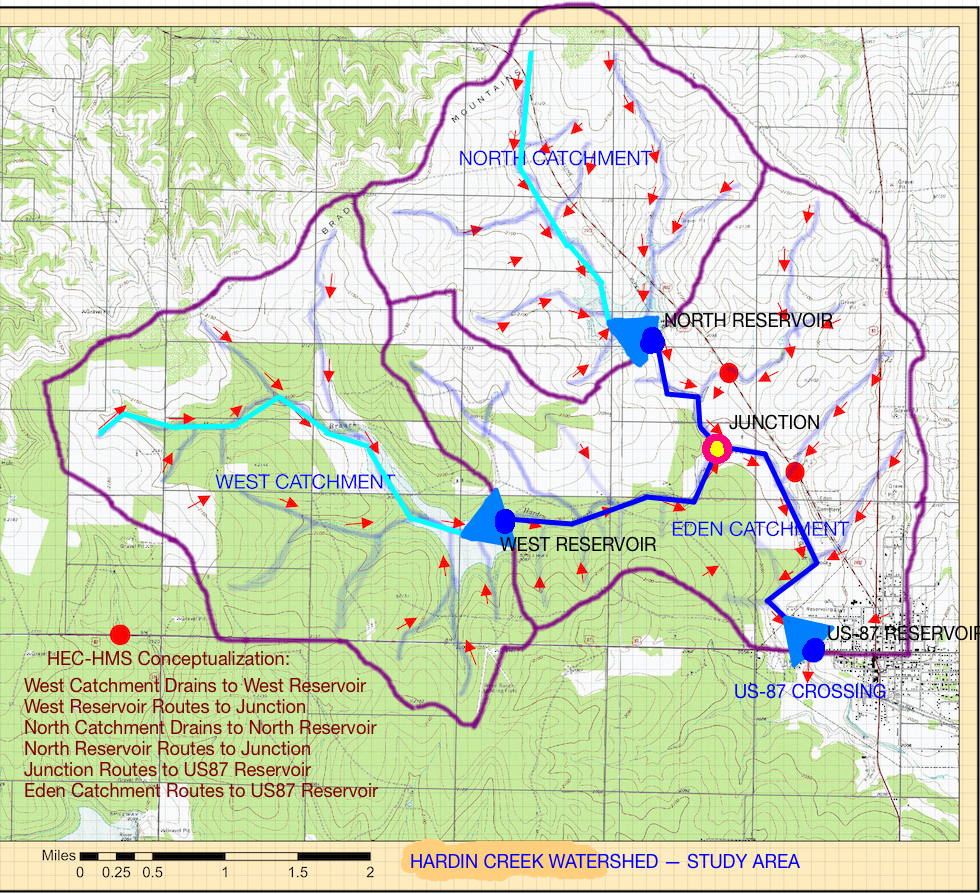
\includegraphics[width=6.0in]{HEC-HMS-Conceptualization.png} 
   \caption{Rocky Run Branch Watershed}
   \label{fig:HEC-HMS-Conceptualization}
\end{figure}
\clearpage

\begin{enumerate}

\item Estimate a basin characteristic time, basin lag or $T_C$, for the Hardin Creek Eden Catchment as depicted in Figure \ref{fig:EdenCatchment} using the Kerby-Kirpich Method, and the NRCS Upland Method.

\begin{figure}[h!] %  figure placement: here, top, bottom, or page
   \centering
   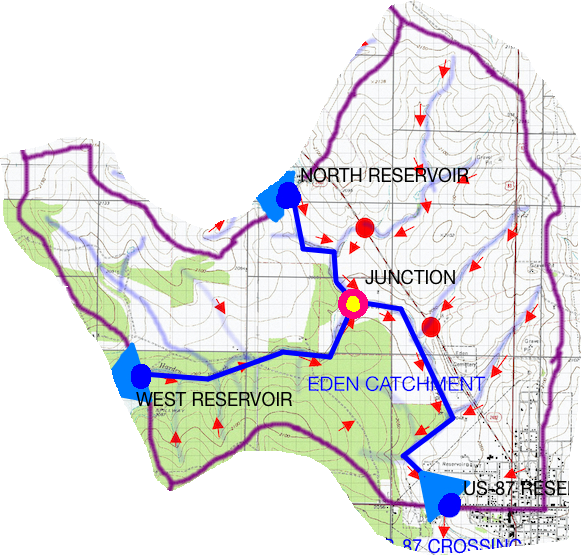
\includegraphics[width=3.0in]{EdenCatchment.png} 
   \caption{Eden Catchment}
   \label{fig:EdenCatchment}
\end{figure}

\item Estimate a basin characteristic time, basin lag or $T_C$, for the Hardin Creek North Catchment as depicted in Figure \ref{fig:NorthCatchment} using the Kerby-Kirpich Method, and the NRCS Upland Method.

\begin{figure}[h!] %  figure placement: here, top, bottom, or page
   \centering
   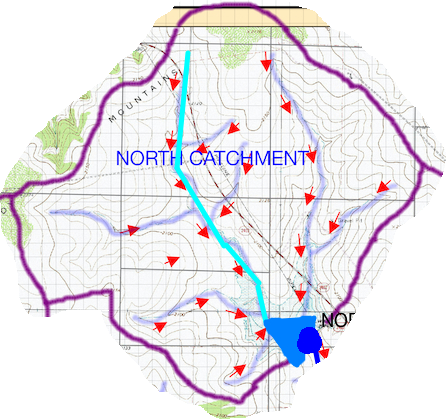
\includegraphics[width=3.0in]{NorthCatchment.png} 
   \caption{North Catchment}
   \label{fig:NorthCatchment}
\end{figure}
\clearpage

\item Estimate a basin characteristic time, basin lag or $T_C$, for the Hardin Creek West Catchment as depicted in Figure \ref{fig:WestCatchment} using the Kerby-Kirpich Method, and the NRCS Upland Method.

\begin{figure}[h!] %  figure placement: here, top, bottom, or page
   \centering
   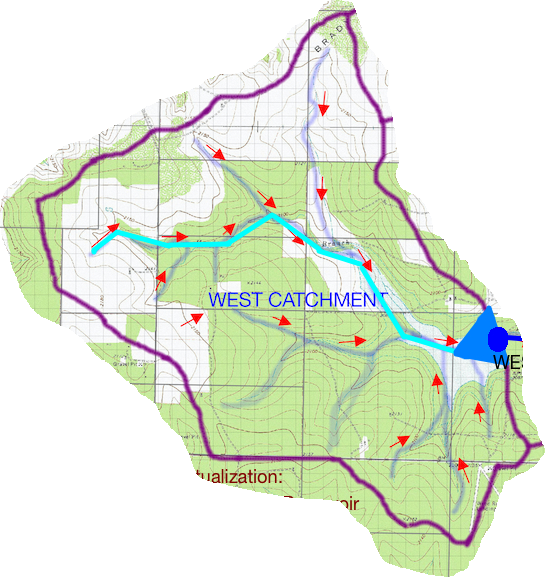
\includegraphics[width=3.0in]{WestCatchment.png} 
   \caption{West Catchment}
   \label{fig:WestCatchment}
\end{figure}

\item Write a brief description of the conceptual relationship of $T_C$ and basin lag time (RSG pp. 364-370)

% Can you describe  the conceptual relationship of basin lag time and the time of concentration in hydrology
%Basin Lag Time

%Basin lag time is the time delay between the peak of the rainfall event and the peak discharge observed at a specific point in the watershed, typically at the outlet. It essentially represents the time it takes for the water from the rainfall event to travel through the watershed and accumulate at the outlet. The lag time is influenced by factors like the basin's shape, size, slope, land use, and soil type.

%Time of Concentration

%Time of concentration is the time it takes for water to travel from the most distant point in the watershed to the outlet, following the longest path. This concept assumes that after this time, the entire watershed contributes to the runoff at the outlet. The time of concentration is a critical parameter in hydrologic modeling, as it helps determine the timing and magnitude of peak flow. It depends on various factors, including the topography, land cover, and flow paths within the basin.

%Relationship

%    Conceptual Sequence: During a rainfall event, water begins to accumulate and flow towards the outlet. The time of concentration marks the moment when runoff from all parts of the watershed has reached the outlet, thus representing the maximum possible flow contribution from the entire basin. The peak discharge generally occurs after this point, with basin lag time marking the delay until this peak is observed.

%    Influence on Hydrograph: The time of concentration helps in determining the shape and timing of the rising limb of the hydrograph, while the basin lag time helps in identifying the time when the peak flow will occur.

%    Calculation and Use: Both parameters are essential for hydrologic modeling and flood forecasting. While time of concentration is often used in determining the design and analysis of drainage systems, basin lag time is useful for flood prediction and understanding watershed response.

%In summary, the time of concentration and basin lag time are related but distinct concepts in hydrology, both describing different aspects of how water travels through a watershed in response to rainfall.

%\item Thornwaithe San Angelo
%\item CN Concho
%\item Green-Ampt concho

\end{enumerate}

\end{document}  